\documentclass[11pt]{article}


\usepackage[sort]{natbib}
\usepackage{bm,amsmath,bbm,amsfonts,nicefrac,latexsym,amsmath,amsfonts,amsbsy,amscd,amsxtra,amsgen,amsopn,bbm,amsthm,amssymb,graphicx}
\usepackage{wrapfig, caption, subcaption}
\usepackage{fancyhdr}
\usepackage[margin=1.0in]{geometry}
\bibliographystyle{abbrvnat}



\title{Fourth Monitoring Committee Meeting \\\vspace{4mm} \normalsize{Understanding the Information Content in Diverse Observations of Forest Carbon Stocks and Fluxes for Data Assimilation and Ecological Modeling\\ NERC case partnership with Forest Research}}
\author{\normalsize{E. Pinnington}}
\date{\normalsize{Room 1L43, 11am June 15, 2015}}


\newtheorem{theorem}{Theorem}[section]
\newtheorem*{defn}{Definition}



	
\begin{document}

\maketitle

\section{Introduction}

Forest ecosystems play an important role in sequestering human emitted carbon-dioxide from the atmosphere and therefore greatly reduce the effect of anthropogenic induced climate change. For that reason understanding their response to climate change is of great importance. Measurements of forest carbon balance are now routinely made in forests across the world using micrometeorological techniques, with many other relevant observations such as leaf area index and standing biomass also available \citep{baldocchi2008turner}. Many efforts have been made to combine this data with models of forest carbon balance using data assimilation techniques in order to improve modelled estimates \citep{fox2009reflex}. Currently, however, the optimal set of observations for understanding the carbon balance of a forest is not known. The aims of this PhD are:

\begin{itemize}
\item Understanding which observations provide models of forest carbon balance with most information in a data assimilation framework, with focus on the case partners research site Alice Holt.
\item Finding a better way to quantify background and observation errors and their correlations.
\item Investigating the effect of disturbance on the Alice Holt research forest. The disturbance came when one side of the forest was thinned and the other side left unmanaged. 
\end{itemize}

Currently we have conducted information content experiments using the Data Assimilation Linked Ecosystem Carbon model (DALEC) \citep{williams2005improved} which have been written up as a report. The report had focused mainly on Shannon Information Content (SIC) and the Degrees of Freedom for Signal (DFS) \citep{rodgers2000inverse} as measures for information content in carbon balance observations. We showed previously that a single observation of the Net Ecosystem Exchange (NEE) of CO$_2$ taken in summer with warmer temperatures and higher daily irradiances had a higher information content than those taken in winter. This made physical sense as in the summer we have more fluxes of carbon through the forest ecosystem, with more photosynthesis and respiration occurring, giving us more information about the fluxes of carbon through our system in summer observations of NEE. In the report on information content this was explored further and it was shown that it would take 30 days of successive NEE observations in winter to give the same amount of information as a single NEE observation made in summer.

DALEC was also implemented in a Four-Dimensional Variational assimilation (4D-Var) scheme and an adjoint model built for state estimation, where our state corresponded to the 5 initial carbon pool values in DALEC. We used this scheme to assimilate observations of NEE with DALEC using data from an evergreen forest in Oregon. It was shown that assimilating NEE observations not only improved our model's estimate of NEE but also improved modelled Gross Primary Production (GPP) and Total ecosystem Respiration (RT). This can be expected as NEE is a product of GPP and RT (NEE = RT - GPP). However, often we see our data assimilation scheme overestimate either GPP or RT and therefore underestimate the other flux when only assimilating NEE. 

Since completing the last report, a new version of the DALEC model was released (DALECV2 \citep{Bloom2014}) and I have built this into a 4D-Var scheme for parameter and state estimation. It was decided to begin work on DALECV2 as it can be parameterised for both deciduous and evergreen forests and the Alice Holt research site is a mainly deciduous forest, whereas the version of DALEC previously used was a model of evergreen forests only. We are currently using data acquired from Alice Holt to run DALECV2 and I have worked on getting the driving data and NEE observations into the right format for use with DALECV2.

I have also now completed taking a set of stem and soil respiration observations for Forest Research at the Alice Holt flux site and am now in the early stages of planning a campaign to take leaf area index measurements at the Alice Holt flux site. I have completed a thesis outline which is included along with the monitoring report.            

\section{DALECV2}

The DALECV2 model is a simple process-based model describing the carbon balance of a forest ecosystem \citep{Bloom2014} and is the new version of the original DALEC \citep{williams2005improved}. The model is constructed of six carbon pools (labile ($C_{lab}$), foliage ($C_f$), fine roots ($C_r$), woody stems and coarse roots ($C_w$), fresh leaf and fine root litter ($C_l$) and soil organic matter and coarse woody debris ($C_s$)) linked via fluxes. The aggregated canopy model (ACM) \citep{williams1997predicting} is used to calculate daily gross primary production ($GPP$) of the forest, taking meteorological driving data and the site's leaf area index (a function of $C_f$) as arguments. A graphical representation of the fluxes in DALECV2 can be seen in figure~\ref{fig:DALEC_mod}.   

\begin{figure}[ht]
    \centering
    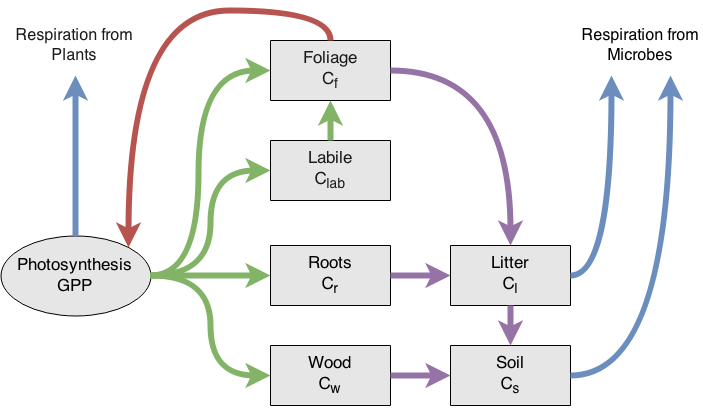
\includegraphics[width=0.5\textwidth]{Dalecdiagram.png}
    \caption{Representation of the fluxes in the DALEC2 carbon balance model. Green arrows represent C allocation, purple arrows represent litter fall and decomposition fluxes, blue arrows represent respiration fluxes and the red arrow represents the feedback of foliar carbon to the $GPP$ function.}
    \label{fig:DALEC_mod}
\end{figure}

\section{4D-Var} \label{4dvar}

In 4D-Var we aim to maximise the probability of our initial state $\textbf{x}_0$ given a set of observations $\textbf{y}$, $P(\textbf{x}_0|\textbf{y})$, over some time window, $N$. $P(\textbf{x}_0|\textbf{y})$ is maximised by minimising a cost function $J(\textbf{x})$ derived from Bayes' Theorem \citep{lewis2006dynamic}. The cost function is given as,

\begin{equation}
J(\textbf{x}_0) = \frac{1}{2}(\textbf{x}_0-\textbf{x}_b)^{T}\textbf{B}^{-1}(\textbf{x}_0-\textbf{x}_b)+\frac{1}{2}\sum_{i=0}^{N}(\textbf{y}_i-h_i(\textbf{x}_i))^{T}\textbf{R}_{i}^{-1}(\textbf{y}_i-h_i(\textbf{x}_i)),
\end{equation}

where $\textbf{x}_b$ is the background and acts as the initial guess to the state $\textbf{x}_0$, $\textbf{B}$ is the background error covariance matrix and quantifies our knowledge of the error in the background, $h_i$ is the observation operator at time $t_i$ and maps the state vector evolved by the nonlinear model ($m_{0\rightarrow i}(\mathbf{x}_{0})=\textbf{x}_i$) to the observations at this time ($\textbf{y}_i$) and $\textbf{R}_i$ is the observation error covariance matrix at time $t_i$ and represents our knowledge of the uncertainty in the observations. The state that minimises the cost function is called the analysis and is denoted as $\textbf{x}_a$, this state is found using a minimisation routine that takes the cost function, the initial guess ($\textbf{x}_b$) and also the gradient of the cost function given as,

\begin{equation}
\nabla J(\textbf{x}_0) = \textbf{B}^{-1}(\textbf{x}_0-\textbf{x}_b)-\sum_{i=0}^{N}\textbf{M}_{i,0}^{T}\textbf{H}_i^{T}\textbf{R}_{i}^{-1}(\textbf{y}_i-h_i(\textbf{x}_i)),
\end{equation}

where $\textbf{H}_i = \frac{\partial h_i(\textbf{x}_i)}{\partial\textbf{x}_i}$ is our linearized observation operator and $\mathbf{M}_{i,0}=\mathbf{M}_{i-1}\mathbf{M}_{i-2}\cdots\mathbf{M}_0$ is our tangent linear model with $\mathbf{M}_i=\frac{\partial m_{i}(\textbf{x}_{i})}{\partial \textbf{x}_{i}}$. We can rewrite the cost function and its gradient to avoid the sum notation as,

\begin{equation}
J(\textbf{x}_0) = \frac{1}{2}(\textbf{x}_0-\textbf{x}_b)^{T}\textbf{B}^{-1}(\textbf{x}_0-\textbf{x}_b)+\frac{1}{2}(\hat{\textbf{y}}-\hat{h}(\textbf{x}_0))^{T}\hat{\textbf{R}}^{-1}(\hat{\textbf{y}}-\hat{h}(\textbf{x}_0)) \label{costfn}
\end{equation}
and
\begin{equation}
\nabla J(\textbf{x}_0) = \textbf{B}^{-1}(\textbf{x}_0-\textbf{x}_b)-\hat{\mathbf{H}}^{T}\hat{\textbf{R}}^{-1}(\hat{\textbf{y}}-\hat{h}(\textbf{x}_0)), \label{gradcostfn}
\end{equation}
where,
\begin{equation}
\hat{\textbf{y}}=
\begin{pmatrix}
\textbf{y}_0 \\
\textbf{y}_1\\
\vdots \\
\textbf{y}_N
\end{pmatrix},
\hspace{1mm}
\hat{h}(\textbf{x}_0)=
\begin{pmatrix}
h_0(\textbf{x}_0) \\
h_1(m_{0\rightarrow 1}(\mathbf{x}_{0}))\\
\vdots \\
h_N(m_{0\rightarrow N}(\mathbf{x}_{0}))
\end{pmatrix},
\hspace{1mm}
\hat{\mathbf{R}}=
\begin{pmatrix}
\mathbf{R}_0 & 0 & 0 & 0 \\
0 & \mathbf{R}_1 & 0 & 0 \\
0 & 0 & \ddots & 0 \\
0 & 0 & 0 & \mathbf{R}_N
\end{pmatrix}
\hspace{1mm} \text{and} \hspace{3mm}
\hat{\mathbf{H}}=
\begin{pmatrix}
\mathbf{H}_0 \\
\mathbf{H}_1\mathbf{M}_0\\
\vdots \\
\mathbf{H}_N\mathbf{M}_{N,0}
\end{pmatrix}.
\end{equation}

\section{4D-Var with DALECV2} \label{sec:4dvardalec}

In our DALECV2 4D-Var scheme the state vector, $\textbf{x}_0$, corresponds to the vector of the 17 model parameters and 6 initial carbon pool values. We use a diagonal approximation to our background and observational error covariance matrices so that, 
$\textbf{B}=\text{diag}(\underline{\sigma}_b^2)$ and $\hat{\textbf{R}}=\text{diag}(\underline{\sigma}_o^2 )$,
where $\underline{\sigma}_b$ and $\underline{\sigma}_o$ are the vectors of the background and observational standard deviations respectively.

In order to find the tangent linear model (TLM) for DALECV2 we need to find the derivative of the model at each time step with respect to the 17 model parameters and the 6 carbon pools. In previous work we were only estimating the 5 initial carbon pool values for DALEC, so the TLM had been calculated by hand. However, now that we are working with a more complex model and are estimating an extra 17 model parameters and 1 initial carbon pool value, we use the AlgoPy automatic differentiation package in Python to calculate the TLM at each time step. This package uses reverse mode automatic differentiation to calculate the derivative of our model. AlgoPy was selected after testing other automatic differentiation packages (PyAutoDiff and ad.py) and finding that AlgoPy could compute the TLM in the fastest time. It is important to test the tangent linear hypothesis as we did with the original DALEC. In 4D-Var we assume the tangent linear hypothesis,
\begin{equation}
m_{0\rightarrow i}(\mathbf{x}_0+\delta\mathbf{x}_0) \approx m_{0 \rightarrow i}(\mathbf{x}_0) + \mathbf{M}_{i,0}\delta\mathbf{x}_0. \label{TLH}
\end{equation}
The validity of this assumption depends on how nonlinear the model is, the length of the assimilation window and the size of the perturbation $\delta\mathbf{x}_0$. We can test the validity for DALECV2 by taking an initial state $\mathbf{x}_0$ and a $5\%$ perturbation for $\delta\mathbf{x}_0$. We then rearrange equation \ref{TLH} to find, 
\begin{equation}
\text{percentage error in TLM} = \begin{vmatrix} \frac{|| m_{0\rightarrow i}(\mathbf{x}_0+\delta\mathbf{x}_0) - m_{0 \rightarrow i}(\mathbf{x}_0) ||}{|| \mathbf{M}_{i,0}\delta\mathbf{x}_0||} - 1 \end{vmatrix} \times 100.
\end{equation}

\begin{figure}[ht]
    \centering
    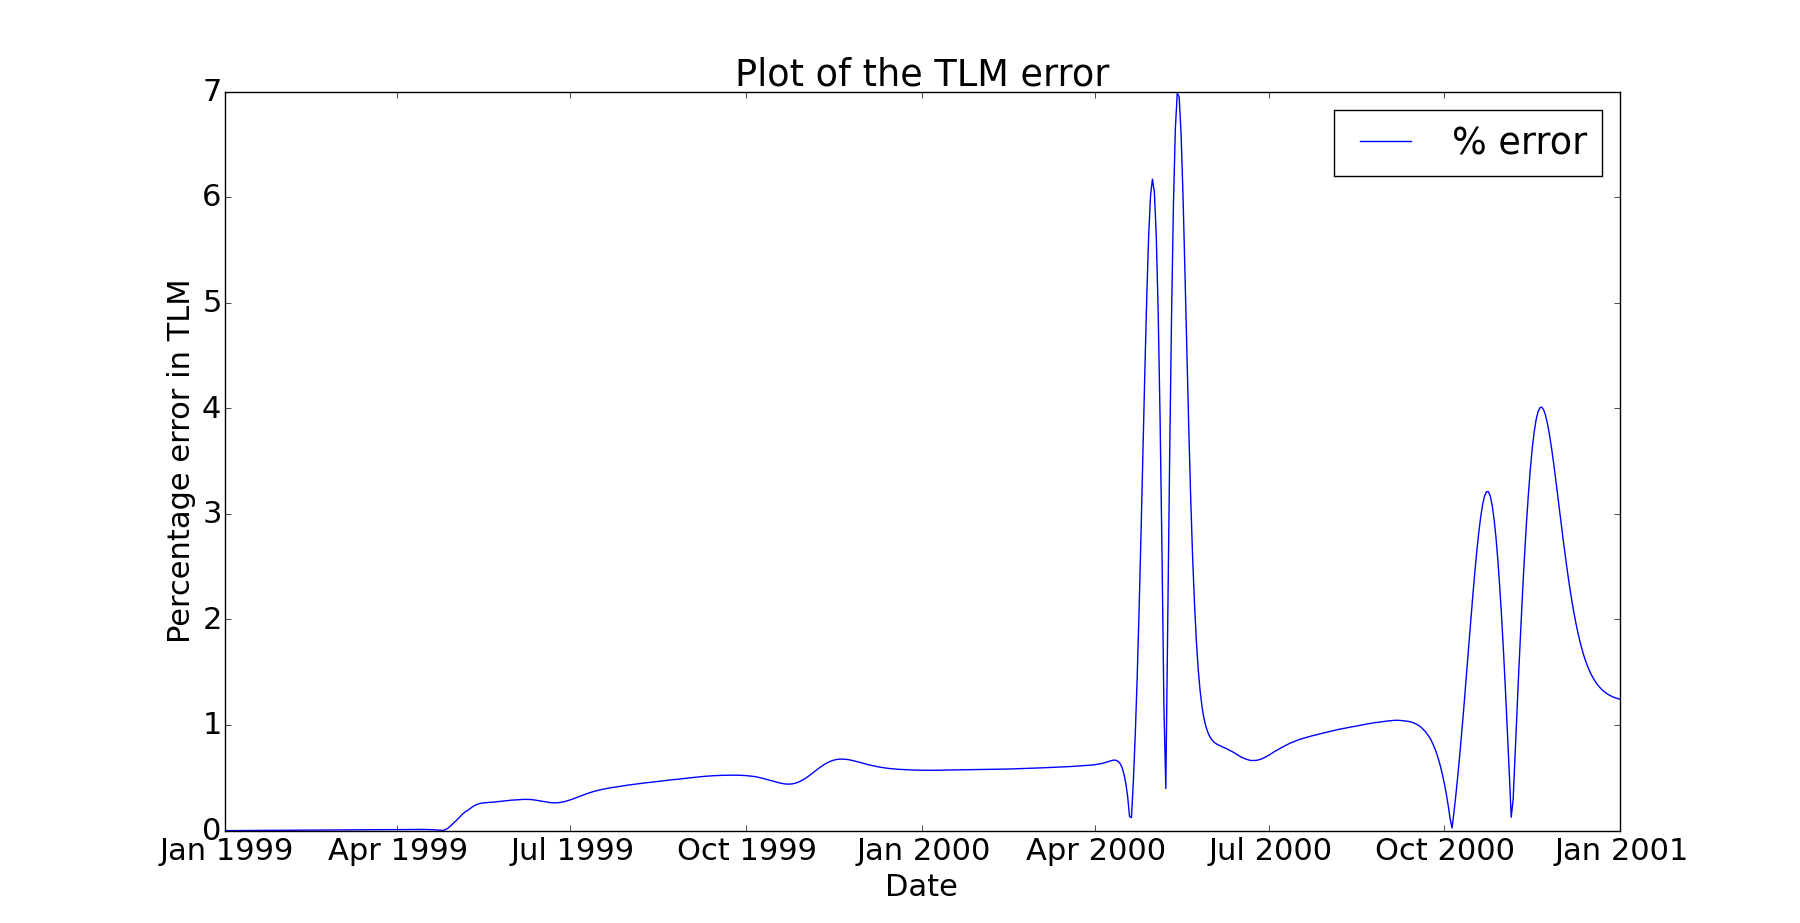
\includegraphics[width=0.6\textwidth]{tlm_error.png}
    \caption{Plot of the percentage error in our tangent linear model for DALECV2 when evolving our state forward over a period of two years.}
    \label{fig:tlm_error}
\end{figure}

In figure \ref{fig:tlm_error} we can see that our TLM for DALECV2 performs very well after being run forward a year with less than a $1\%$ error. By the second year, we see some peaks in our error in spring and autumn; this is where functions controlling leaf on and leaf off in the nonlinear DALECV2 have gone out of phase with the TLM, as the TLM diverges from the nonlinear model. Even at these peaks our error is still reasonable, reaching a maximum at $7\%$ and then coming back to around $1\%$. It was also shown that for the relative error,
\begin{equation}
E_r = \frac{|| m_{0\rightarrow i}(\mathbf{x}_0+\gamma\delta\mathbf{x}_0) - m_{0 \rightarrow i}(\mathbf{x}_0) ||}{|| \mathbf{M}_{i,0}\gamma\delta\mathbf{x}_0||},
\end{equation}
$E_r \rightarrow 0$ as $\gamma \rightarrow 0$. We also performed tests for the gradient of the cost function and for the adjoint model.

In figure~\ref{fig:4dvar} we see a 4D-Var run using NEE observations and meteorological driving data from Alice Holt. Here we are using a truncated Newton method \citep{Nocedal1999} from the Python package Scipy.optimize to find the minimum of our 4D-Var cost function. Our $\textbf{x}_b$ is a parameter set found by the University of Edinburgh using the CARbon DAta-MOdel fraMework (CARDAMOM) \citep{Exbrayat2015}. This used Harmonised World Soil Database $C_{s}$ observations as initial conditions, meteorological driving data from ERA-interim and Markov chain Monte Carlo techniques to assimilate MODIS leaf area index observations over a 10 year period. 

\begin{figure}[!h]
    \centering
    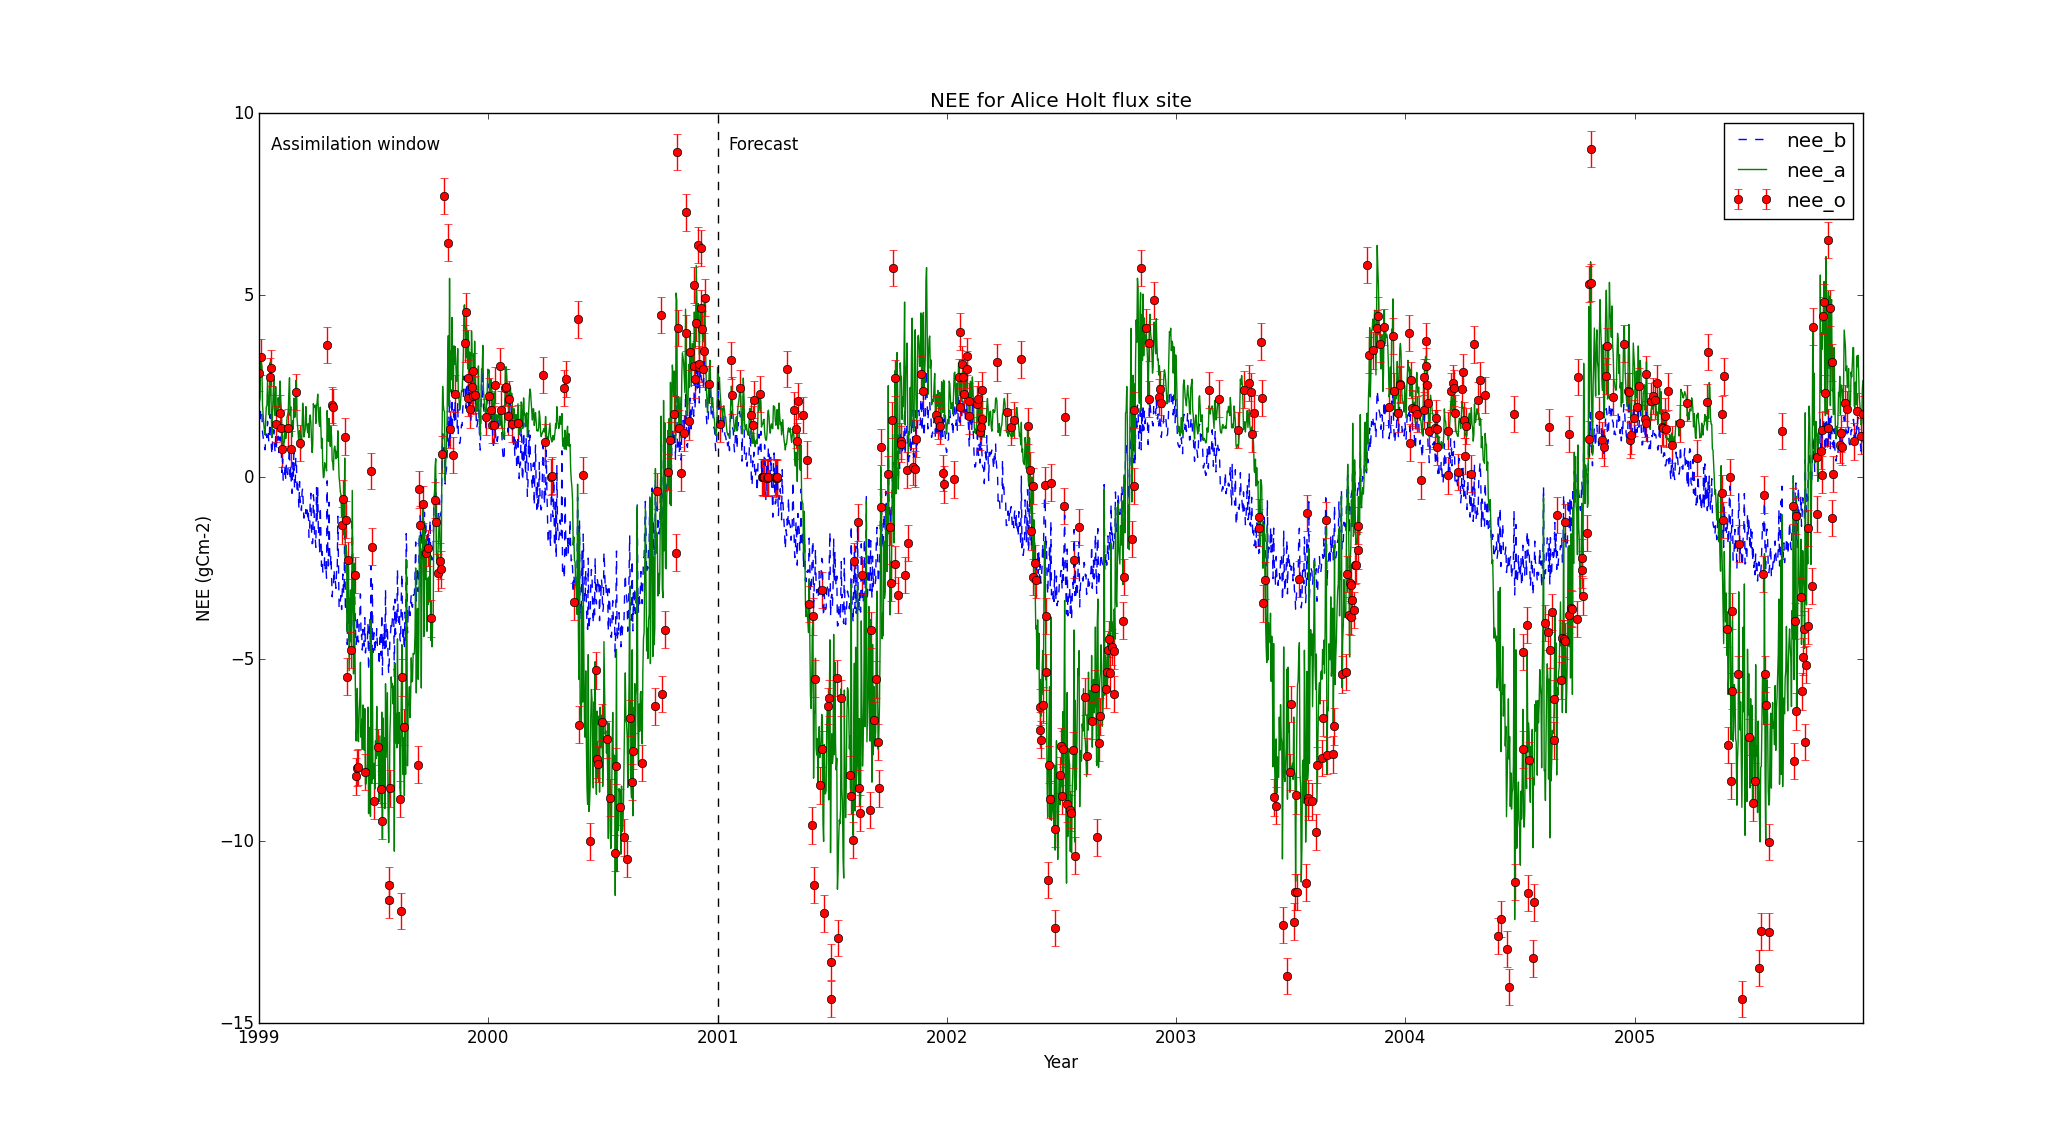
\includegraphics[width=.9\textwidth]{ah_assim_edinpvals.png}
    \caption{4D-Var run for Alice Holt flux site, assimilating NEE observations from 1999-2001 and then forecasting NEE from 2001-2006. The red dots are our observations, the blue dotted line our background estimate and the green line is the model run for the whole period from the analysis.}
    \label{fig:4dvar}
\end{figure}

From figure~\ref{fig:4dvar} we can see that after assimilating NEE observations from 1999-2001 and then running our analysis forward from 2001-2006, we have a much better forecast of NEE than we did from our initial background guess (when judging against observations). However our analysis run is still failing to recreate some of the extreme observations, this may be because we have assimilated 2 years of data with less extreme negative values of NEE. We can see the improvement and reduction in error from figure~\ref{fig:neeobs}. After assimilation we have reduced the error in our forecast by a factor of 2, with our background forecast having a root mean square error of $4.37 \text{gCm}^{-2}\text{day}^{-1}$ and our analysis forecast a root mean square error of $2.12 \text{gCm}^{-2}\text{day}^{-1}$ between the model and observations. It can be seen from figure~\ref{fig:neeobs} that our background forecast constantly under predicts the more negative values of NEE while our analysis forecast has a better spread around the 1:1 line.

\begin{figure}[!h]
\centering
\begin{subfigure}{.5\textwidth}
  \centering
  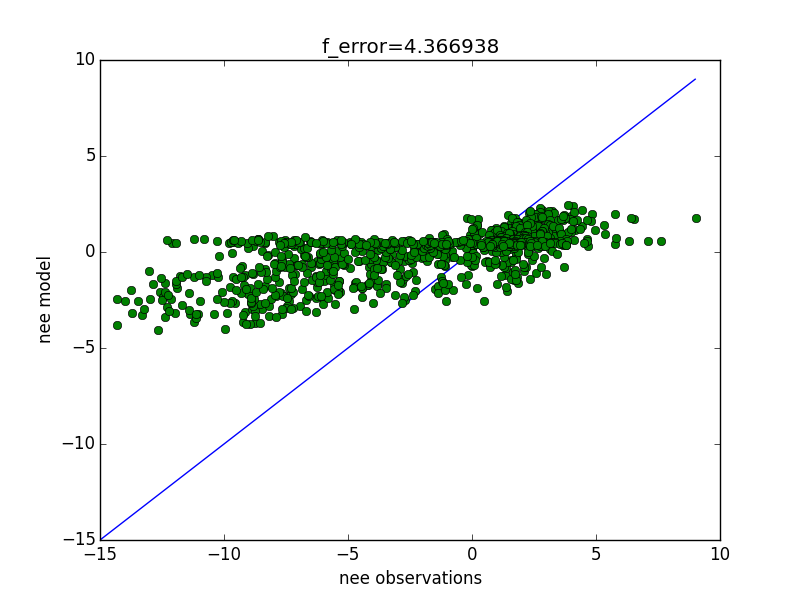
\includegraphics[width=.7\linewidth]{scatterobsvsmodfb.png}
  \caption{Background forest with error of $4.37 \text{gCm}^{-2}\text{day}^{-1}$}
  \label{fig:sub1}
\end{subfigure}%
\begin{subfigure}{.5\textwidth}
  \centering
  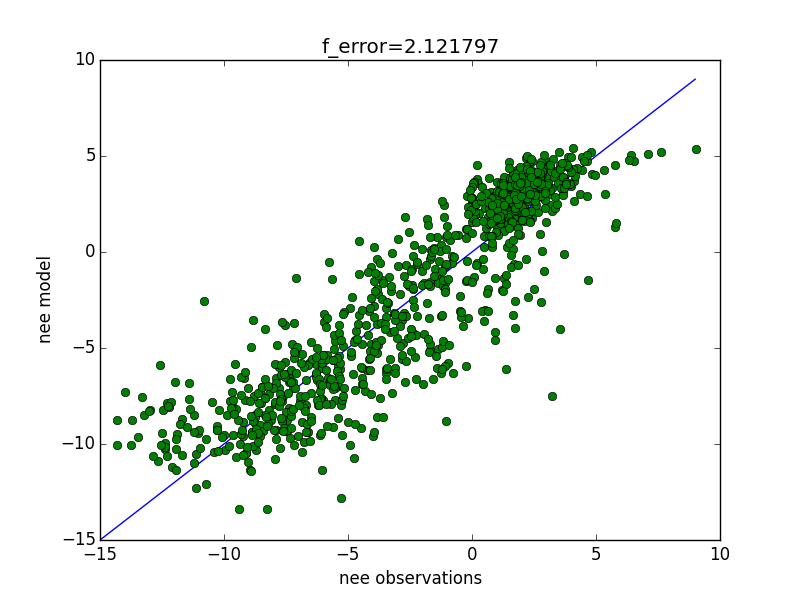
\includegraphics[width=.7\linewidth]{scatterobsvsmodfa.png}
  \caption{Analysis forecast with error of $2.12 \text{gCm}^{-2}\text{day}^{-1}$}
  \label{fig:sub2}
\end{subfigure}
\caption{Scatter plots of forecast NEE against observations of NEE (years 2001-2006) for the Alice Holt flux site. Root mean square error is given in the title of each plot.}
\label{fig:neeobs}
\end{figure}

\section{Current Work and Future Plans}

I am currently writing a report on 4D-Var with DALECV2 using the Alice Holt observations and driving data with a view to produce a paper on the subject.

I am also repeating the information content experiments now using DALECV2. While applying the measures previously used (SIC and DFS), I am also starting to work with the influence matrix, which measures the sensitivity of the analysis in observation space to the observations \citep{Cardinali2004}, and the adjoint technique proposed by \cite{Langland2004}, which approximates the sensitivity of a scalar forecast error norm to the observations. In \cite{Cardinali2004} the data assimilation problem is assumed to be Gaussian with a linear function mapping the state to observation space (\textbf{H}), such that,
\begin{equation}
\textbf{x}_{a} = \textbf{x}_{b} + \textbf{K}(\textbf{y} - \textbf{H}\textbf{x}_{b}), \label{daupdate}
\end{equation}
where \textbf{K} is the Kalman gain matrix, $\textbf{K} = (\textbf{H}^{T}\textbf{R}^{-1}\textbf{H} + \textbf{B}^{-1})^{-1}\textbf{H}^{T}\textbf{R}^{-1}$. The influence matrix is then defined as,
\begin{equation}
\textbf{S} = \frac{\partial {\mathbf{H}}\textbf{x}_a}{\partial {\textbf{y}}} = \textbf{K}^{T}\textbf{H}^{T}. \label{influmat}
\end{equation}
In order to consider observations over a 4D-Var time window we rewrite equation~\ref{daupdate} as,
\begin{equation}
\textbf{x}_{a} = \textbf{x}_{b} + \hat{\textbf{K}}(\hat{\textbf{y}} - \hat{\textbf{H}}\textbf{x}_{b}), \label{ass_xa}
\end{equation}
using the defined matrices in section~\ref{4dvar}, with $\hat{\textbf{K}} = (\hat{\textbf{H}}^{T}\hat{\textbf{R}}^{-1}\hat{\textbf{H}} + \textbf{B}^{-1})^{-1}\hat{\textbf{H}}^{T}\hat{\textbf{R}}^{-1}$. Equation~\ref{influmat} then becomes,
\begin{equation}
\textbf{S} = \frac{\partial {\hat{\mathbf{H}}}\textbf{x}_a}{\partial \hat{{\textbf{y}}}} = \hat{\textbf{K}}^{T}\hat{\textbf{H}}^{T}. \label{influmat2}
\end{equation}
In equation~\ref{ass_xa} we have also assumed that we have a linear model, $\mathbf{M}_{i,0}$, evolving our state from time 0 to time $i$. We know that our model is in fact nonlinear but have tested the tangent linear hypothesis for DALECV2 in section~\ref{sec:4dvardalec} and have seen it to be a good approximation. 

In figure~\ref{fig:nee_IM} we have plotted the influence matrix for 365 days of NEE observations using equation~\ref{influmat2} and our DALECV2 4D-Var scheme. Here 0 corresponds to the $1^{\text{st}}$ January and 365 to the $31^{\text{st}}$ December, we can see that the observations from day 150 to day 250 (roughly June to September) are the observations that have most influence on our analysis in observation space. This is as expected from previous experiments using SIC and DFS. 

\begin{figure}[!ht]
    \centering
    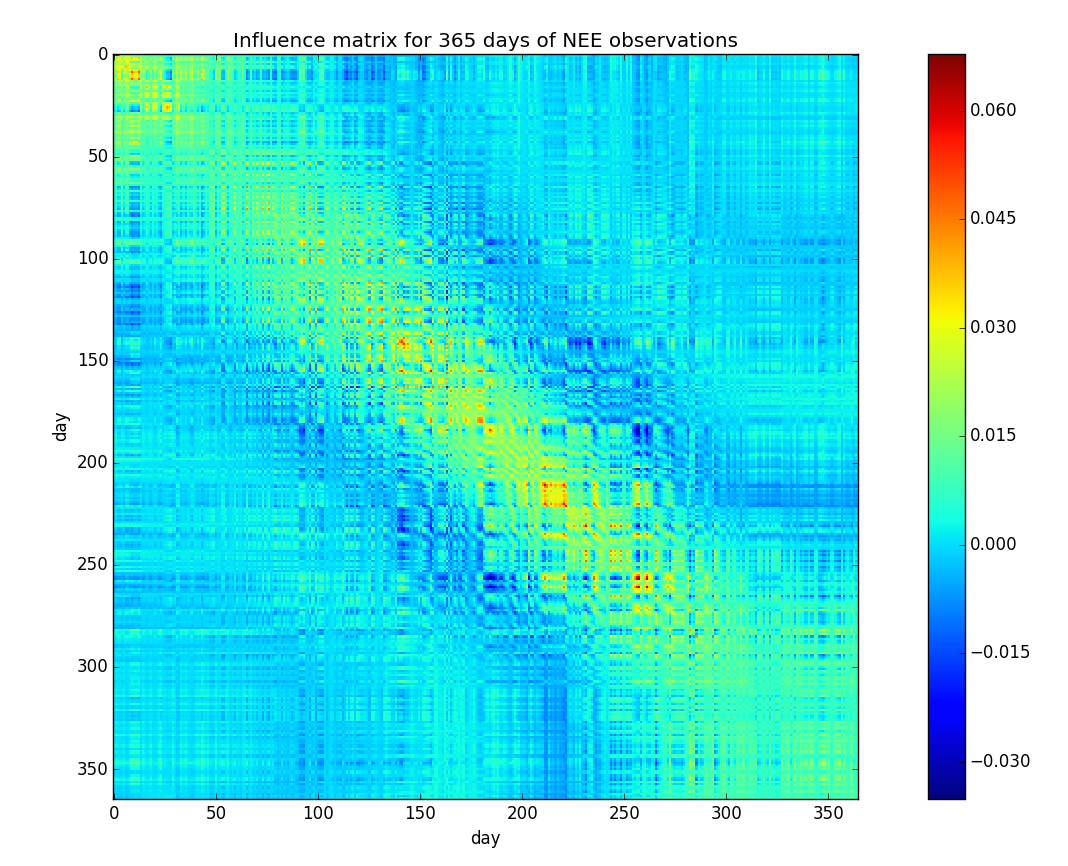
\includegraphics[width=.5\textwidth]{365days_nee.png}
    \caption{Influence matrix as defined in equation~\ref{influmat2} for a years worth of daily NEE observations.}
    \label{fig:nee_IM}
\end{figure}

Using these measures and an observing system simulation experiment that I have developed, I will produce another report investigating the best set of observations for understanding the carbon balance of a forest and apply the results to the available data from Alice Holt. 

I am also in the very early stages of planning a fieldwork campaign at Alice Holt. In this campaign I will be taking measurements of leaf area index using a ceptometer and hemispherical photographs. These measurements will be taken along transects of the forest. The ceptometer allows for quick measurements meaning all transects could be measured within a day. Hemispherical photographs are slower taking around a week to measure all transects. For this reason we will primarily use the ceptometer for our measurements with the hemispherical photographs used as a point of comparison. Tristan and I have a meeting with Forest Research on the $28^{th}$ May to further plan the fieldwork. These measurements will be used in the information content experiments but also to address site specific science questions. Half of the Alice Holt forest has been thinned and the other half left unmanaged.  The flux tower measuring NEE is placed directly on the boundary of the two halves. The leaf area index measurements will allow us to compare the difference between the two sides and also evaluate DALECV2's estimate of leaf area index. We will also parameterise two versions of DALECV2 for the thinned/unthinned forest using NEE observations and a tower foot print model to split the NEE observations when the signal is coming from the thinned or unthinned side of the forest. We will then be able to see if by just assimilating NEE we can pick out a difference in leaf area index between the two sides.

Other future work will be based on the attached thesis outline. This includes attempting to improve the representation of background and observational error covariance matrices in DALECV2. We will use the Desroziers diagnostic for estimating \textbf{B} and \textbf{R} \citep{desroziers2005diagnosis}. As we often only have one observation of NEE at anytime in our assimilation the Desroziers diagnostic will be expanded to allow us to consider correlations in time, in a similar way as we have expanded the definition of the influence matrix, \textbf{S}, earlier in this section. Improving our estimates of \textbf{B} and \textbf{R} is important as improving our representation of these matrices could lead to different results in the information content experiments and ultimately improve the results from our data assimilation experiments. 



\section{Professional and Academic Development}

\subsection{Masters Courses}
\begin{itemize}
\item MAMB10 (Data Assimilation) - 85\%
\item MAMNSO (Numerical Solutions to Ordinary Differential Equations) - 79\%
\item MTMG02 (Atmospheric Physics) - 66\%
\item MTMG49 (Boundary Layer) - 72\%
\item MTMD01 (Environmental Data Visualization) - 78\%
\item MTMD02 (Operational Data Assimilation) - 70\%
\end{itemize}

\subsection{Transferable Skills}

During my PhD I have taken part in the following courses, workshops and activities:
\begin{itemize}
\item 28/01/2014 - Basic Statistics Refresher - RRDP

\item 31/03/2014-01/04/2014 - Land Data Assimilation workshop at UCL - ESA

\item 23/04/2014-25/03/2014 - Correlated Observation Errors in Data Assimilation Workshop - ESA

\item 13/05/2014 - Social Media - Bloggs, Twitter and Your Online Presence - RRDP

\item 29/05/2014 - How to Write a Paper - RRDP

\item 25/06/2014-26/06/2014 - Software Carpentry Course - Git and Python

\item 10/07/2014-11/07/2014 - Forest Research - Helped with field work LiDAR

\item  21/07/2014-01/08/2014 - Fluxcourse Summer School - University of Colorado

\item 29/09/2014-03/10/2014 - NERC course - Software Development for Environmental Scientists Level 1

\item 08/10/2014-10/10/2014 - Environment YES - NERC ``dragon's den" type competition at Syngenta, Jesops Hill

\item 17/12/2014 - Presentation at Maths for Planet Earth Industry day

\item 24/02/2015 - Reading Soil Centre Workshop - What can Land Surface Models do for you?

\item 23/03/2015-27-03/2015 - NERC course - Software Development for Environmental Scientists Level 2
\end{itemize}

\subsection{Demonstrating}
During my PhD I have helped demonstrate on the following courses:
\begin{itemize}
\item 15/09/2014-1909/2014 - NERC Data assimilation for environmental scientists training course

\item 16/02/2015-20/02/2015 - NERC Software Development for Environmental Scientists Level 1

\item 20/04/2015-23/04/2015 - MT26E Surface Energy Exchange Practicals
\end{itemize}


\bibliography{../../PhD}{}
%\bibliographystyle{plain}
\end{document}